\documentclass[a4paper, 12pt]{article}

\usepackage[T2A]{fontenc}
\usepackage[utf8]{inputenc}

\usepackage[english, russian]{babel}

\usepackage{amsmath, amsfonts, amsthm, mathtools, amssymb}
\usepackage[left = 1cm, top=10mm, right=20mm, bottom=0.6cm, bindingoffset=0cm]{geometry}
\usepackage{setspace}
\setstretch{1.2}
%Рисунки
\usepackage{graphicx}
\usepackage{wrapfig }
\usepackage{multirow}
\renewcommand{\arraystretch}{1.5}

\begin{document}
\begin{titlepage}
	\centering
	{\scshape\LARGE Московский физико-технический институт \par}
	\vspace{10cm}
	{\scshape\Large Лабораторная работа 3.2.3 \par}
	\vspace{1cm}
	{\huge\bfseries Резонанс токов в параллельном контуре \par}
	\vspace{1cm}
	\vfill
\begin{flushright}
	{\large выполнили студенты группы Б03-302}\par
	\vspace{0.3cm}
	{\LARGE Пазов Тенгиз, Симухин Егор}

\end{flushright}
	\vfill
% Bottom of the page
	25.10.2024 г.
\end{titlepage}
\large\section{Цель работы:}
\hspace{0.6cm}Исследование резонанса напряжений в последовательном колебательном контуре с
изменяемой ёмкостью, включающее получение амплитудно-частотных и фазово-частотных характеристик, а также определение основных параметров контура.

\section{Оборудование:}
\hspace{0.6cm}Генератор сигналов, источник напряжения, нагруженный на последовательный колебательный контур с переменной ёмкостью, двулучевой осциллограф, цифровые вольтметры.

\section{Экспериментальная установка}
\hspace{0.6cm}Схема экспериментального стенда для изучения резонанса токов в параллельном колебательном контуре показана на рис. 1а. Синусоидальный сигнал от генератора GFG-8255A поступает на вход источника тока, собранного на операционном усилителе ОУ с полевым транзистором ПТ, питание которых осуществляется встроенным блоком-выпрямителем от сети переменного
тока 220 вольт. Цепи питания на схеме не показаны, представлен только резистор , переменное напряжение на котором в используемой схеме равно напряжению на входе «+» операционного усилителя. Источник тока, обладающий по определению бесконечным внутренним сопротивлением, фактически обеспечивает постоянство амплитуды тока на меняющейся по величине нагрузке – параллельном контуре, изображенном на рис. 1. в виде эквивалентной схемы. На рис. 1б контур представлен почти в натуральную величину. Источник тока, колебательный контур и блок питания заключены в отдельный корпус с названием «Резонанс токов» на верхней крышке, отмеченный на рисунке штриховой линией. На корпусе имеются коаксиальные разъёмы «Вход», «$U_{1}$» и «$U_{2}$», а также переключатель магазина ёмкостей с указателем номера n = 1, 2, ... 7. Величины ёмкостей и сопротивления
, указаны в табличке на крышке корпуса. Напряжение поступает на вход
«+» операционного усилителя от генератора через согласующую RC-цепочку. Это же напряжение через разъём «$U_{1}$» подаётся одновременно на канал 1 осциллографа GOS-620 и вход 1-го цифрового вольтметра GDM-8245. Переменное напряжение на резисторе $R_{1}$, как отмечалось выше, при этом также равно Е. Напряжение на контуре U, совпадающее с напряжением на конденсаторе, подаётся со знаком «–» через разъём «$U_{2}$» на канал 2 осциллографа и вход 2-го цифрового вольтметра GDM-8245. Показанные на схеме установки ещё два конденсатора без наименований (помимо входящего в RC-цепочку) играют вспомогательную роль и не влияют на характеристики контура. Символ «→ +» отмечает наличие источника питания полевого транзистора. Колебательный контур нашей установки собран из стандартных элементов, используемых в
современных радиоэлектронных цепях. Известно, что в реальных конденсаторах и, особенно, в катушках индуктивности происходят необратимые потери энергии, обусловленные различными причинами. К ним относятся: утечки и диэлектрические потери в конденсаторах, вихревые токи и потери на перемагничивание в сердечниках катушек индуктивности, омические потери в проводниках, растущие с частотой за счёт скин-эффекта, и некоторые другие. Рост потерь приводит к увеличению действительных частей комплексных сопротивлений элементов контура, и, значит, к изменению его резонансных свойств, в частности, к уменьшению добротности. Потери в элементах контура зависят как от частоты, так и от амплитуды тока (напряжения),
температуры и ряда других факторов, например, от вида диэлектрика конденсатора, сердечника катушки и т.д. От перечисленных факторов в общем случае зависят и основные параметры контура: индуктивность L, ёмкость C и суммарное активное сопротивление.


\begin{center}
\begin{figure}[ht]
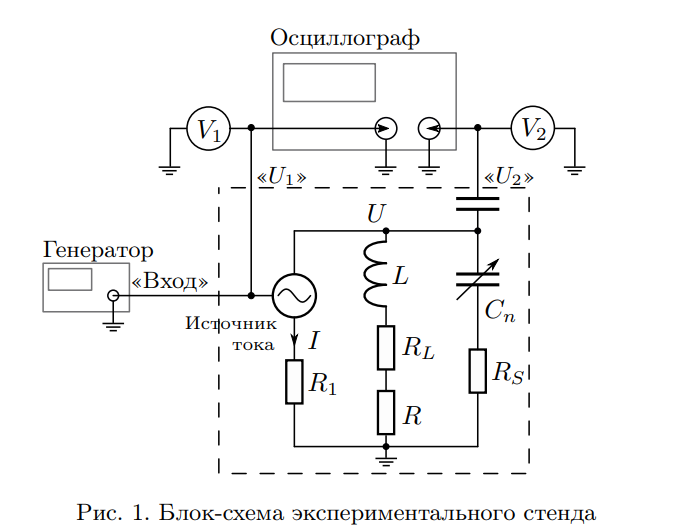
\includegraphics[width = 1\textwidth]{Снимок экрана 2024-10-25 191509.png}
\caption{Схема установки}
\end{figure}
\end{center}

\section{Теоретические сведения:}
\hspace{0.6cm}
\begin{equation}
$I=\dfrac{E}{R_I}=\dfrac{E_0cos(\omega t+\varphi_0)}{R_I}=I_0cos(\omega t+\varphi_0)$ --- ток на генераторе\newline
$$R_S=\dfrac{U_{RS}}{I}=\frac{U_{RS}}{\omega CU_{CS}}=\dfrac{1}{\omega C}tg\delta$$
где $R_S$ - эквивалентное последовательное сопротивление (ЭПС)\newline
Для используемых емкостей $C_n$ выполнено $tg\delta<10^{-3}$\newline
$$R_{\sum}=R+R_L+R_S$$
где $R_{\sum}$ - суммарное активное сопротивление контура.\newline
Воспользуемся методом комплексных амплитуд:\newline
$Z_L=R_L+i\omega L$, $Z_C=R_S-i\frac{1}{\omega C}$, $Z=R_{\sum}+i(\omega L-\dfrac{1}{\omega C})$\newline
Тогда напряжение на контуре и токи на индуктивной и емкостной частях контура при нулевой начальной фазе можно предствить в виде:\newline
$$I_c=I\dfrac{Z_L}{Z_C+Z_L}=iQI_0\dfrac{\omega}{\omega_0}\dfrac{1-i\dfrac{R+R_L}{\rho}\dfrac{\omega_0}{\omega}}{1+iQ(\dfrac{\omega}{\omega_0}-\dfrac{\omega_0}{\omega})}$$
$$I_L=I\dfrac{Z_c}{Z_C+Z_L}=iQI_0\frac{\omega_0}{\omega}\frac{1+itg\delta}{1+iQ(\frac{\omega}{\omega_0}-\frac{\omega_0}{\omega})}$$
$$U=I\frac{Z_LZ_c}{Z_C+Z_L}=Q\rho I_0\frac{(1-i\frac{R+R_L}{\rho}\frac{\omega_0}{\omega})(1+itg\delta)}{1+iQ(\frac{\omega}{\omega_0}-\frac{\omega_0}{\omega})}$$
где $\omega_0=\frac{1}{\sqrt{LC}}$ - собственная частота, $\rho=\sqrt{\frac{L}{C}}$ - реактивное сопротивление контура, $Q=\frac{\rho} - {R_{\sum}}$ - добротность контура\newline
Рассмотрим случай, когда $|\Delta\omega|=|\omega-\omega_0|\ll\omega_0$. Тогда
$$\frac{\omega}{\omega_0}-\frac{\omega_0}{\omega}=\frac{2\Delta\omega}{\omega_0}$$
Пренебрегая поправками порядка $Q^{-2}$, получим:
$$I_c=QI_0\frac{\omega}{\omega_0}\frac{e^{i\phi_c}}{\sqrt{1+(\tau\Delta\omega)^2}},    \phi_c=\frac{\pi}{2}-\frac{R+R_L}{\rho}-arctg(\tau\Delta\omega)$$
$$I_L=QI_0\frac{\omega_0}{\omega}\frac{e^{i\phi_L}}{\sqrt{1+(\tau\Delta\omega)^2}}, \phi_L=-\frac{\pi}{2}+\delta\arctg(\tau\Delta\omega)$$
$$U=Q\rho I_0\frac{\omega}{\omega_0}\frac{e^{i\phi_U}}{\sqrt{1+(\tau\Delta\omega)^2}}, \phi_U=-\frac{\omega}{\omega_0}\frac{R+R_L}{\rho}+\delta-arctg(\tau\Delta\omega)$$
где $\tau=\frac{2L}{R_{\sum}}=\frac{2Q}{\omega_0}$ - время затухания.\newline
При резонансе, т.е. когда $\Delta\omega=0$:
$$I_c(\omega_0)=QI_0, \phi_c(\omega_0)=\frac{\pi}{2}-\frac{R+R_L}{\rho}$$
$$I_L(\omega_0)=QI_0, \phi_L(\omega_0)=-\frac{\pi}{2}+\delta$$
$$U(\omega_0)=Q\rho I_0=Q^2R_{\sum}I_0, \phi_U{\omega_0}=-\frac{R+R_L}{\rho}+\delta$$
$$\phi'_c(\omega_0)=\phi'_L(\omega_0)=\phi'_U(\omega_0)=-\tau$$
\end{equation}
\section{Обработка данных}

\begin{table}[h!]
	\begin{tabular}{|c|c|c|c|c|c|c|c|c|c|c|c|}
		\hline
		$n$ & $C_n$, нФ & \begin{tabular}[c]{@{}c@{}}$f_{0n}$, \\ кГц\end{tabular} & $U_C$, В & $E$, В & \begin{tabular}[c]{@{}c@{}}$L$, \\ мкГн\end{tabular} & $Q$ & \begin{tabular}[c]{@{}c@{}}$\rho$, \\ Ом\end{tabular} & \begin{tabular}[c]{@{}c@{}}$R_{\sum}$, \\ Ом\end{tabular} & \begin{tabular}[c]{@{}c@{}}$R_{S_{\max}}$,\\ Ом\end{tabular} & $R_L$, Ом & $|Z_{rez}|$, кОм \\ \hline
		1 & 22,0 & 34,34 & 1,41 & 0,2488 & 977,37 & 25,32 & 210,77 & 8,32 & 0,21 & 4,20 & 5,34 \\ \hline
		2 & 33,1 & 28,06 & 0,98 & 0,2490 & 972,92 & 21,56 & 171,44 & 7,95 & 0,17 & 3,87 & 3,70 \\ \hline
		3 & 47,9 & 23,58 & 0,71 & 0,2498 & 952,05 & 19,20 & 141,00 & 7,34 & 0,14 & 3,30 & 2,70 \\ \hline
		4 & 57,4 & 21,30 & 0,59 & 0,2504 & 973,67 & 17,27 & 130,24 & 7,54 & 0,13 & 3,50 & 2,25 \\ \hline
		5 & 66,7 & 19,74 & 0,51 & 0,2508 & 975,57 & 16,07 & 120,94 & 7,52 & 0,12 & 3,49 & 1,95 \\ \hline
		6 & 82,1 & 17,781 & 0,42 & 0,2517 & 976,84 & 14,68 & 109,08 & 7,43 & 0,10 & 3,41 & 1,60 \\ \hline
            7 & 99,6 & 16,112 & 0,36 & 0,2530 & 980,67 & 13,83 & 99,00 & 7,17 & 0,10 & 3,17 & 1,37 \\ \hline
	\end{tabular}
	\caption{Измерение резонансных частот и характеристик контура}
	\end{table}

 \begin{table}[h!]
    \centering
    \begin{tabular}{|c|c|c|}
    \hline
            & L, мкГн & $R_L$, Ом \\ \hline
            Среднее значение & 972.73 & 3.56 \\ \hline
            Среднеквадратичная погрешность & 9,47 & 0.36\\ \hline
 	\end{tabular}
	\caption{Измерение погрешностей для L и $R_{L}$}
\end{table}
Оценим вклад активных потерь в кондесаторе $\dfrac{R_{S_{max}}}{R_{\sum}} = \dfrac{\rho \cdot 10^{-3}}{R_{\sum}} < 2.9\%$

Оценим влияние погрешности приборов на ход эксперимента. При построении графика зависимости $R_{l}(f_{0n})$ были взяты погрешности, указанные в методичке - 3 \% для U и 1 \% для f.
Для 3-его и 5-ого конденсаторов построим на одном графике амплитудно-частотные характеристики в координатах f, $U_{c}(f)$ (рис. 2)

Далее построим на одном графике амплитудно-чатсотные характеристики в безразмерных координатах для этих же конденсаторов $x = f/f_0, y = U_{c}(f)/U_{c}(1)$.
По ширине резонансных кривых на уровне 0,707 определим добротности Q соответствующих контуров (рис. 2)
Соответсвенно для контуров 3 и 5 получили $Q_{5} = 16,82 \pm 0,02, Q_{3} = 19,87 \pm 0,03$. Из таблицы 1 видно, что добротности для данных контуров не совпали с полученными из безразмерного графика y(x). Однако они совпадают в пределах первого порядка.
\text{ при } x = 1$ (рис. 4)
\begin{figure}[h!]
\begin{center}
  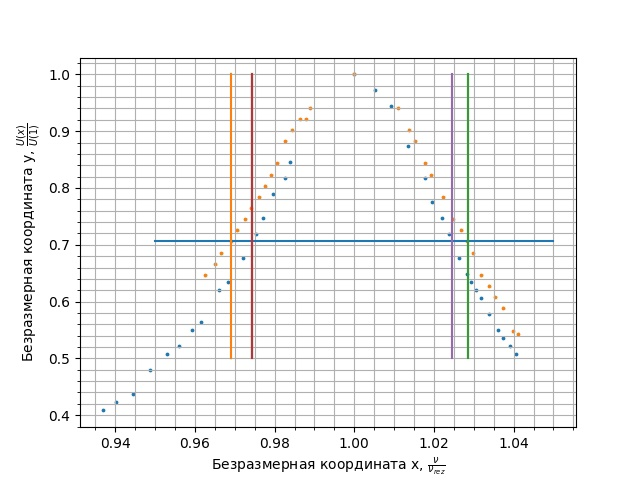
\includegraphics[width = 1\textwidth]{jJB4E4wzxKuGV_tEMkuDArz5UldAfYsEJytjUuL7MSHnwpxdwG0k2O6ar_IJf8JQcXOIKiW3mhcx4C-HPjPHD0tj.jpg}
  \end{center}
  \vspace{-0.5cm}
  \caption{АЧХ}
\end{figure}
%\newpage
%\begin{figure}[h!]
  %\begin{center}
    %\includegraphics[width = 1\textwidth]{График ФЧХ в относительных единицах.png}
  %\end{center}
  %\vspace{-0.5cm}
  %\caption{ФЧХ в относительных единицах}
%\end{figure}
По данным табл. 1 построим зависимость $R_{L}(f_{0n})$ и нанесем прямую $\langle R_{L} \rangle$. 
\begin{figure}[h!!]
  \begin{center}
    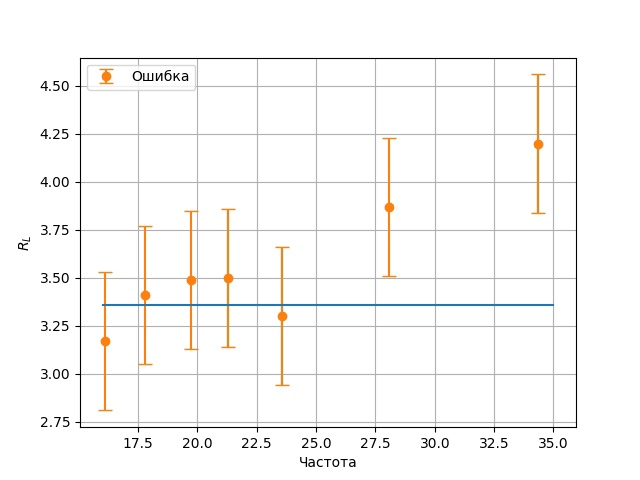
\includegraphics[width = 1\textwidth]{1TaWn49QNAc.jpg}
  \end{center}
  \vspace{-0.5cm}
  \caption{Зависимость напряжения на катушке от резонансной частоты}
\end{figure}
Проанализировав оба графика, получились следующие значения для добротности и погрешностей.
Построим векторную диаграмму тока и напряжений для тока с наименьшей добротностью в резонансном состоянии.

\begin{figure}[h!]
  \begin{center}
    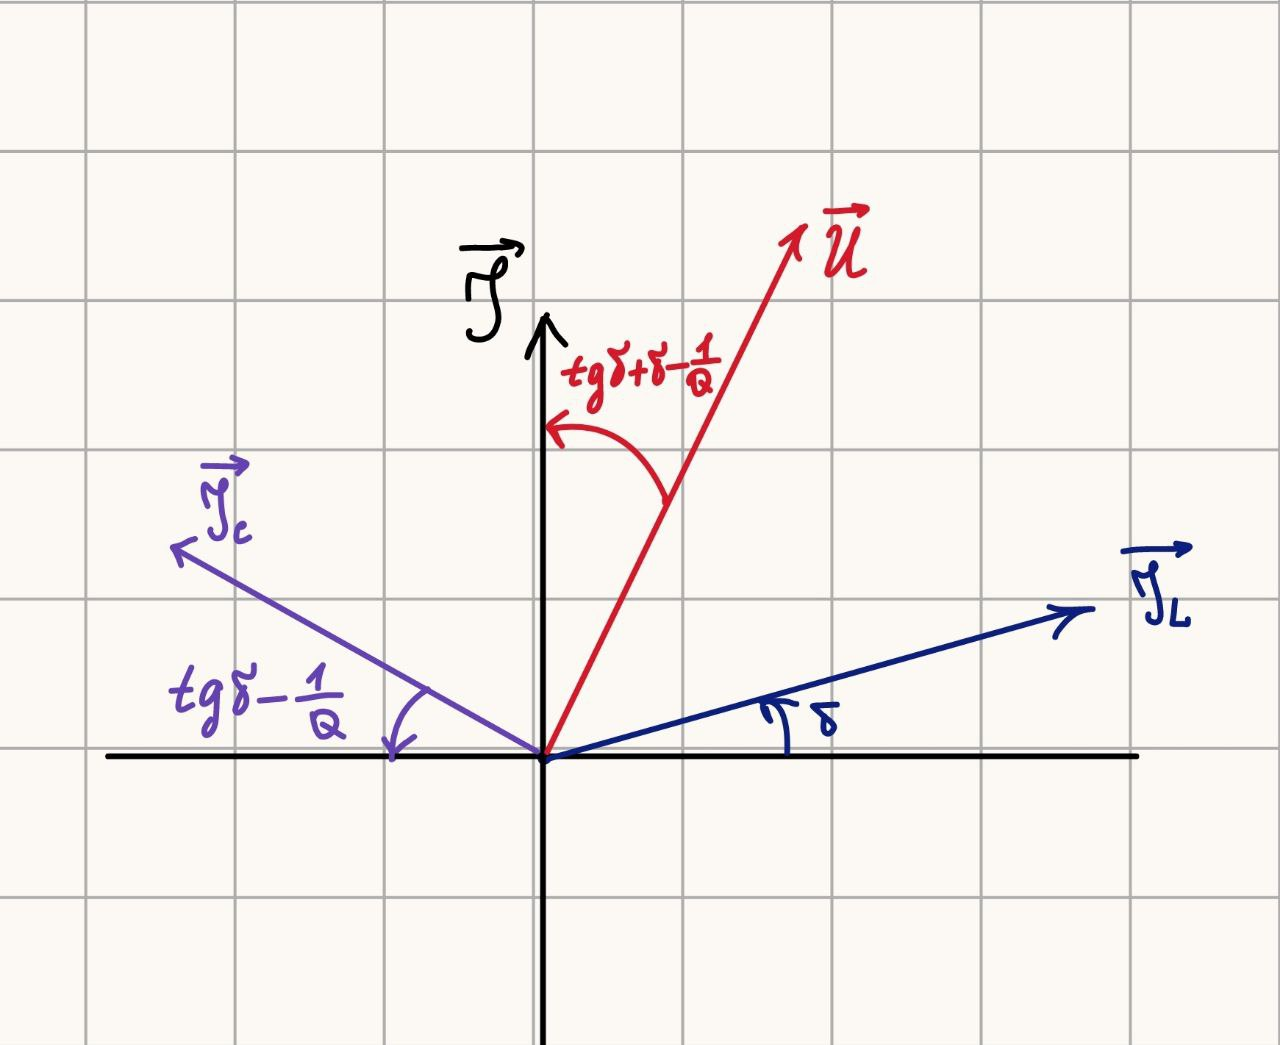
\includegraphics[width = 1\textwidth]{1.jpg}
 \end{center}
 \vspace{-0.5cm}
  \caption{Векторная диаграмма}
\end{figure}
Также построим ФЧХ, основываясь на результатах эксперимента.
\newpage
\begin{figure}[h!]
  \begin{center}
    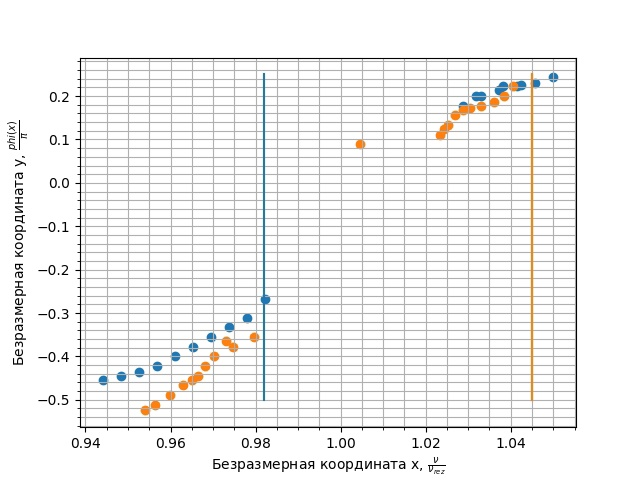
\includegraphics[width = 1\textwidth]{3WpWcuqtU_s.jpg}
  \end{center}
  \vspace{-0.5cm}
  \caption{ФЧХ в относительных единицах}
\end{figure}
\begin{center}
\begin{figure}[ht]
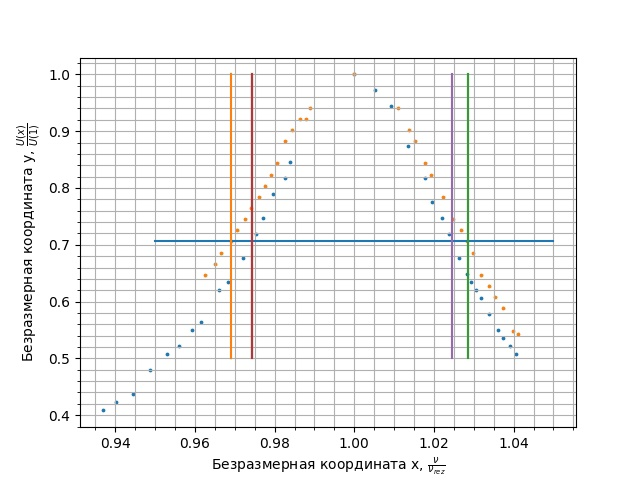
\includegraphics[width = 1\textwidth]{jJB4E4wzxKuGV_tEMkuDArz5UldAfYsEJytjUuL7MSHnwpxdwG0k2O6ar_IJf8JQcXOIKiW3mhcx4C-HPjPHD0tj.jpg}
\caption{АЧХ}
\end{figure}
\end{center}
Построили ФЧХ, из которого мы не можем сделать выводов о добрротности контура N=5 в силу отсутствия экспериментальных точек в интересующем нас диапазоне по оси y(-1/4; 1/4). Однако можно сделать вывод о добротности контура N=3 так как хватает экспериментальных измерений. Добротность была найдена как $Q = \frac{1}{\Delta x}$, где $\Delta x$ - расстояние между точками оси x, в которых $\phi / \pi$ меняется от -1/4 до 1/4. Q = 14,49.
\begin{table}[h!]
\centering
\begin{tabular}{|l|ll|ll|}
\hline
\multirow{}{}{} & \multicolumn{2}{l|}{С3}     & \multicolumn{2}{l|}{С5}     \\ \cline{2-5} 
                  & \multicolumn{1}{l|}{Q} & $\sigma_{Q}$ & \multicolumn{1}{l|}{Q} & $\sigma_{Q}$ \\ \hline
АЧХ               & \multicolumn{1}{l|}{19,87} & 0,02   & \multicolumn{1}{l|}{16,82}  & 0,03  \\ \hline
ФЧХ               & \multicolumn{1}{l|}{14,49}  &  0,261 & \multicolumn{1}{l|}{---}  &  ---  \\ \hline
Расчитанные       & \multicolumn{1}{l|}{19,20}  &    & \multicolumn{1}{l|}{16,07}  &    \\ \hline
\end{tabular}
\caption{Значение добротностей полученных из графиков АЧХ и ФЧХ}
\end{table}
\section{Вывод}
Был изучен резонанс токов в параллельном rlc контуре. Активные потери в конденсаторе, а также погрешность измерительных приборов мало влияют на результаты эксперимента. Были построены амплитудно-частотные и фазово-частотные характеристики для двух конденсаторов. Была измерена различными способами добротность контура - результаты измерений при разных способах совпадают в пределах погрешности. Также была получена зависимость сопротивления катушки от частоты при резонансе в контуре с наименьшей добротностью: зависимость получилась линейной, что говорит о сильной завышенности погрешности. О причинах такой зависимости авторы не догадываются. Была построенная векторная диаграмма, на которой графически показано, что при резонансе векторы $I_{c}$, $I_{L}$ в сумме дают вектор I.
\end{document}
